%%%%%%%%%%%%%%%%%%%%%%%%%%%%%%%%%%%%%%%%%%%%%%
\section{Run Plan}
\label{sec:runplan}

To formulate a preliminary run plan, we assume the hadron beam spectrum and rates are as given in Tables~\ref{tab:beampartcomp} and~\ref{tab:beampartrates}.   For the purpose of estimating the sample composition and beam time request, the following assumptions are used:
\begin{itemize}
\item { Trigger/date rate = 25~Hz}
\item { Two 4.8 sec spills per SPS Super Cycle }
\item { SPS Super Cycle = 48 sec}
\item { Particle ID trigger for electron is available}
\item { Trigger rate for electron in hadron beam is prescaled to 0.5~Hz}
\end{itemize}
We plan to run the H4 beamline in two modes: the first configuration is optimized for the production of hadrons and the second configuration is optimized for the production of high purity electrons. Even in the hadron mode, the beam is still dominated by electrons, especially for low beam momenta. However, the electrons in the hadron beam are not particularly ``clean'' due to the amount of materials in the beamline from the particle identification (PID) instrumentations .  The proposal is to heavily prescale the electron events using PID (e.g. Threshold Cherenkov counters) trigger while running in hadron mode. The PID systems that contribute significantly to the material budget will be removed when we reconfigure the beamline for electron beam.  We are exploring various run plan scenarios. One of the scenarios is shown in Tables~\ref{tab:HadRunPlan} and ~\ref{tab:ElecRunPlan}. 
\begin{cdrtable}[Run Plan]{ccccccccc}{HadRunPlan}{A preliminary run plan for ProtoDUNE-SP hadron beam. The expected sample (positive beam) as a function of momentum is shown. }
P & \# of  &\# of $e^+$ & \# of $K^+$ & \# of $\mu^+$ & \# of $p$ & \# of $\pi^+$ & Total \# & Beam Time \\ 
(GeV/c) & Spills  & &  &  &  &  & of Events & (days) \\ \toprowrule
1 & 70K & 84K & $\approx$ 0 & 13K  & 672K & 504K & 1.3M & 19 days\\ \colhline
2 & 20K & 24K & 8K & 21K     & 336K & 480K & 0.9M &5.6 days\\ \colhline
3 & 12K & 14K & 14K  & 14K   & 163K & 516K  & 720K & 3.3 days\\ \colhline
4 & 10K & 12K & 23K & 15K    & 90K  & 460K & 600K & 2.8 days\\ \colhline
5 & 10K & 12K  & 25K  & 6K   & 81K  & 475K & 600K & 2.8 days\\ \colhline
6 & 10K & 12K & 34K  & 5K    & 82K  & 468K & 600K & 2.8 days\\ \colhline
7 & 10K & 12K & 34K & 7K     & 80K  & 467K & 600K & 2.8 days\\ \colhline
 & & & & & & & \\
Total & 142K & 170K & 132K & 81K & 1.5M & 3.4M & 5.3M & 39 days\\
\end{cdrtable}
\begin{cdrtable}[Run Plan]{cccc}{ElecRunPlan}{A preliminary run plan for ProtoDUNE-SP electron beam. The expected sample for positive beam configuration is shown. }
Momentum Bins (GeV/c) & \# of Spills per Bin & \# $e^+$ per Bin & Beam Time (days) per Bin \\ \toprowrule
0.5, 06, 0.7, 0.8, 0.9, 1, 2, 3, 4, 5, 6, 7 & 5000 & 300K & 1.4 days \\
\end{cdrtable}

Tables with similar values are expected for the negative beam sample. 

Preliminary beam simulations show that the hadron rates at 
energies below 1~GeV/c are low. Moreover, low-energy beams are more
subject to disruption and degradation by materials in the
beamline.  Therefore, the beam program factors in both the beam composition and %also takes into account of 
particle interaction topologies.  Full FLUKA\cite{fluka05,Fluka15}
 simulations
of particle transport in the the ProtoDUNE-SP detector, including the
beam window, have been performed.
 The physics requirement \fixme{that the beam must satisfy overall? Anne} is %the possibility 
 to enable measurement of
 stopping particles and  interactions at both high and low energies.    
%
At a beam momentum of 1~GeV/c, 35\% of protons stop, while the percentage reduces to only 5

per mill at 2~GeV/c. 
\fixme{use same units, \% or per mill (per thousand?)}  At  1~GeV/c,  the protons interact at all
energies as shown in
Figure~\ref{fig:pandpiint}. 
\fixme{protons of all energies interact? Anne}
The residual energy at the interaction
point can be reconstructed by measuring the energy deposited along the proton track.
Many of the  low-energy pions decay in the 37~m between the secondary target
and the LAr volume.  The fraction of stopping $\pi$'s for one $\pi$
leaving the target is 3\% at $p=0.4$~GeV/c,  %still  
1.3\% at $p=0.7$~GeV/c,
then decreases.  Having a $\pi$ beam at 0.7~GeV/c still allows 
measurement of pion interactions down to few tens of MeV with good
statistics. In a 1-GeV/c beam, the low-energy interactions are %still
present, albeit at a %with 
lower rate, as shown in Figure~\ref{fig:pandpiint}.
%
As for kaons, the length of the beamline is such that no
$K$ arrives at the detector for momenta lower than $\approx$2~GeV/c.
\fixme{``no $K$ with momentum lower than $\approx$2~GeV/c arrives at the detector'' Anne}
As for electrons, the peculiar topology of very low-energy electron-initiated 
showers requires a measurement at the lowest possible momenta.
\begin{cdrfigure}[Energy at interaction]{pandpiint}{Kinetic energy of
    particles at the point of interaction in the ProtoDUNE-SP active
    volume, for different beam momenta. Histograms are normalized to one particle injected in the
    beamline acceptance. FLUKA simulations include the beam window
    materials, beams are considered as monochromatic and
    parallel. Left: protons, Right: pions.}
  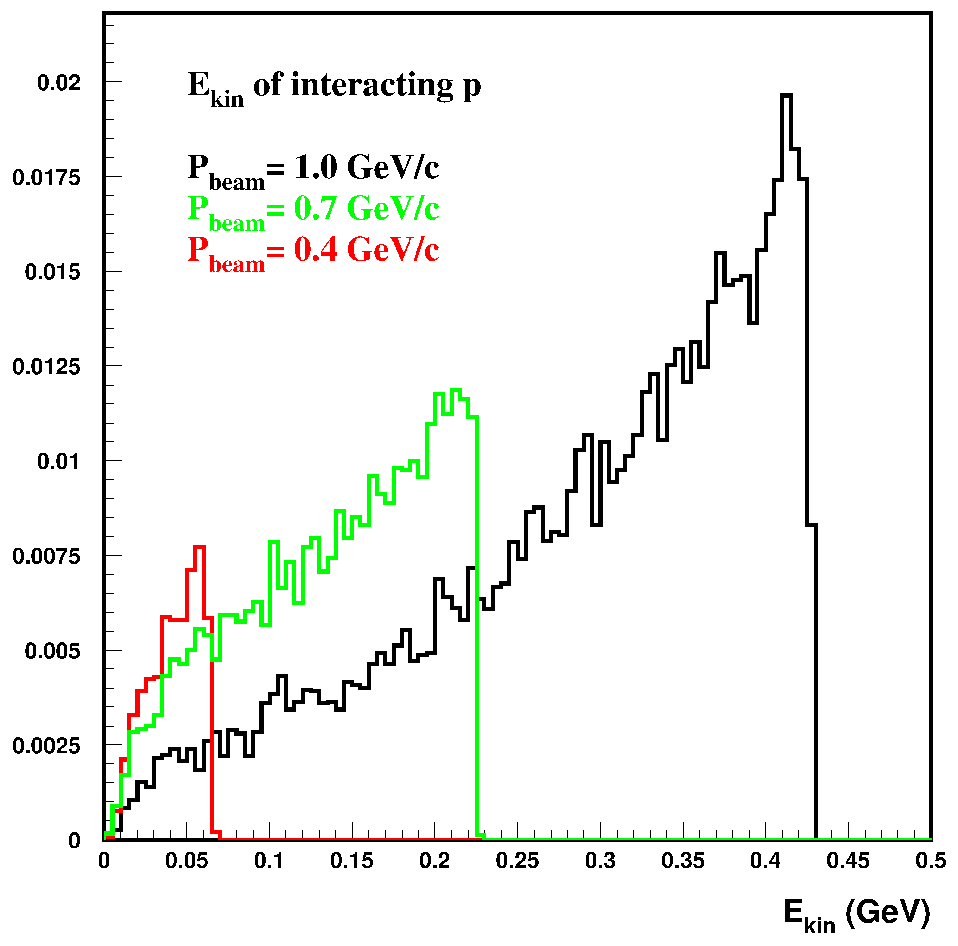
\includegraphics[width=0.49\textwidth]{pvarie_intene.pdf}
  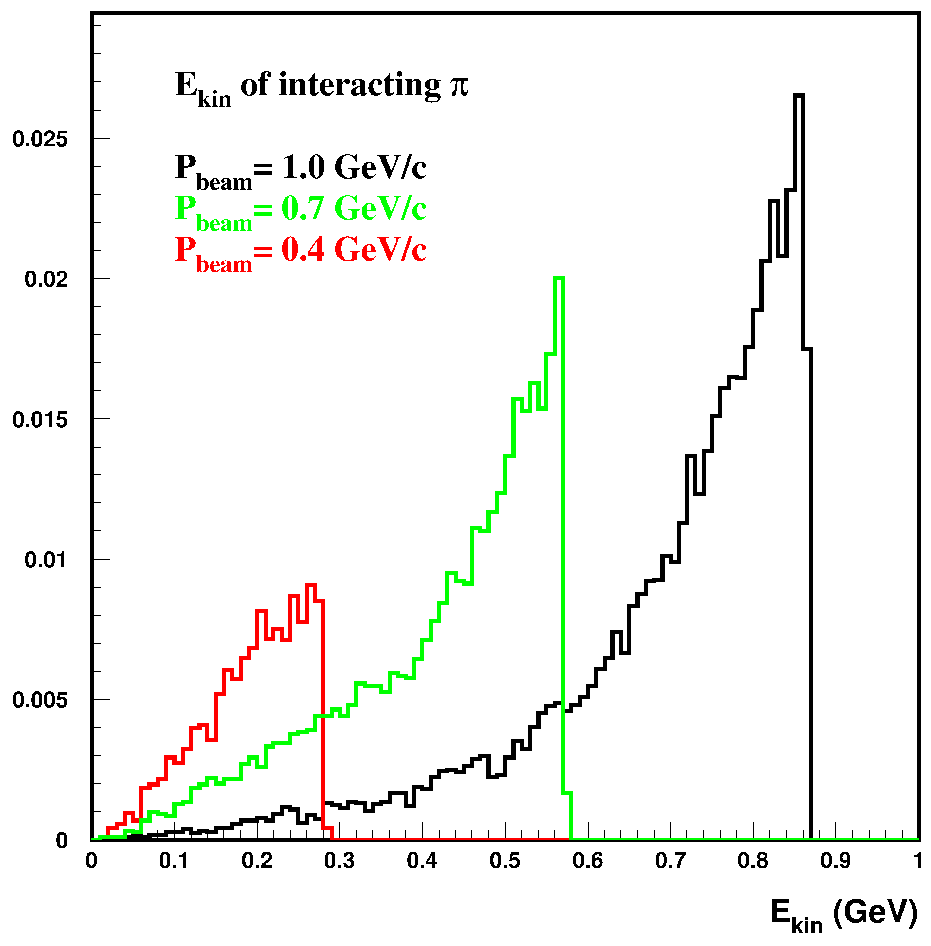
\includegraphics[width=0.49\textwidth]{pivarie_intene.pdf}
\end{cdrfigure}
%% end of   part that can go either here or in the run plan 

Based on the current information available, the total estimated beam time needed to carry out the physics program in this proposal with the assumptions stated earlier is on the order of 16 weeks.
 
 



